\pagebreak
\subsection{Manipulación}

A continuación vamos a experimentar que tan manipulable es el algoritmo PageRank a medida que va cambiando el factor de teletransportacion. La idea es la siguiente, un algoritmo con un factor de teletransportacion bajo pondera menos en la matriz de transición el componente que representa la estructura del grafo. Por lo tanto, un Search Engine que tenga este factor de teletransportacion bajo va a ser sumamente manipulable, dado que puedo crear muchisimos nodos e inflar el ranking de cualquier sitio. Cuanto mayor es este factor, conjeturamos que vamos a observar que inflar cualquier sitio sera mucho mas costoso en termino de cantidad de sitios únicos que debo crear. De hecho, Page \& Brin en su paper consideran esto y mencionan que en Google se ponderan muchos factores para evitar lo que hoy se conoce como SEO (Search Engine Optimization).

Primero vamos a ver las posiblidadades de manipulación con $c = 0.85$. Para hacer esto se fijo el valor de $c$, y se tomo una red inicial de 30 nodos y 30 ejes, y a la primer pagina se le agrego una pagina que la apunte por cada iteracion, este proceso se repitio hasta agregar 80 enlaces a la primer pagina. El resultado es:

\begin{figure}[H]
\centering
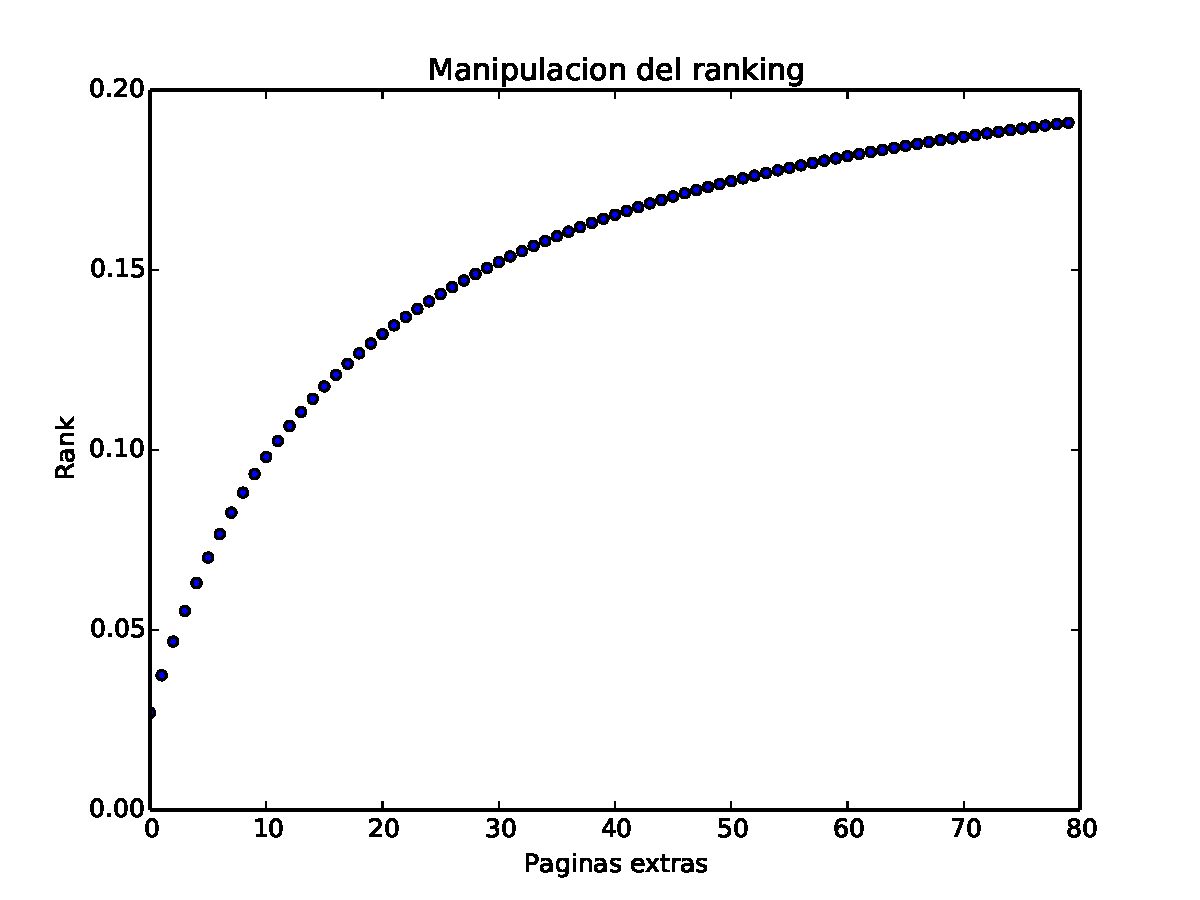
\includegraphics[scale=0.7]{images/manipulacion.pdf}
\caption{Score de una pagina web a medida que creamos mas paginas que lo apuntan.}
\label{timePageRank}
\end{figure}


Como era de esperar, a medida que aumentamos el numero de sitios web que apuntan a otro, su ranking comienza a subir lentamente. Sin embargo, el beneficio marginal de agregar nuevos sitios web es decreciente. Esto se debe a que la relevancia que aporta un nuevo sitio al que nadie lo linkea depende de forma decreciente de la cantidad de sitios web totales.

El aporte de un nuevo sitio web de este estilo siempre mejorara o mantendra el ranking de un sitio web. Aunque la relevancia total depende de todos los sitios que lo linkean, y al agregar un sitio le estoy quitando relevancia a los sitios web originales que lo linkeaban, el incremento en la relevancia al agregar un nuevo sitio web con $c$ fijo compensa la caida en la relevancia de los sitios originales. Por eso observamos una curva creciente. Sin embargo, el beneficio marginal de agregar un sitio web luego solo compensa por la perdida en relevancia del resto de los sitios, razon por la cual la sucesion dada por la cantidad de nuevos sitios web parece converger.

Para el ultimo caso (es decir, el caso con los nuevos 80 enlaces extras apuntando a la primer pagina), decidimos ver como influyen los valores de $c$ en su ranking. Se tomo $c = 0$, se lo aumento en $0.1$, hasta llegar a $0.9$. La idea es que a medida que aumenta c, el factor de teletransportacion tiene una mayor relevancia en el ranking de un sitio web. Por ejemplo, sabemos que si $c = 1$, se ignora la estructura del grafo y todos los sitios web tendran la misma relevancia, dado que todos linkean a todos con la misma probabilidad. El resultado fue el siguiente:

\begin{figure}[H]
\centering
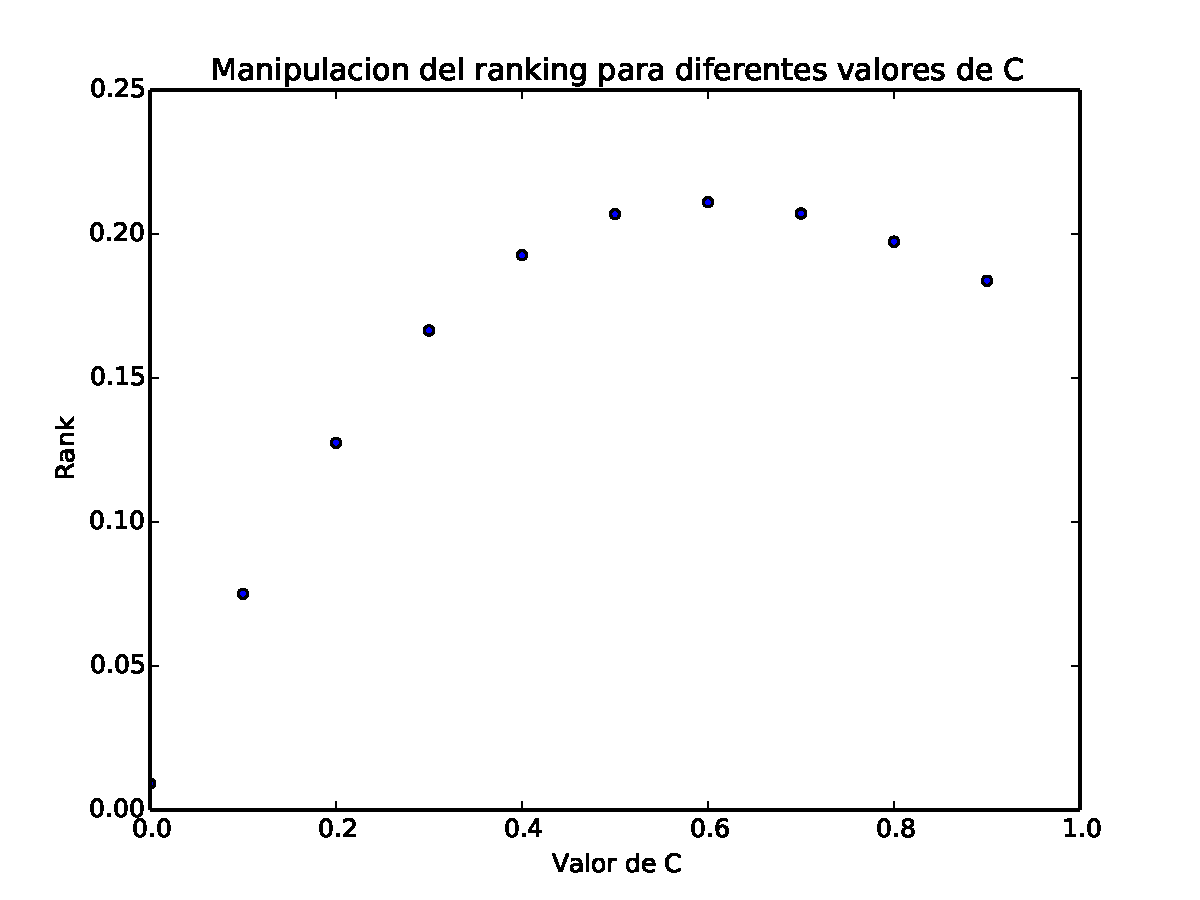
\includegraphics[scale=0.7]{images/manipulacionC.pdf}
\caption{Cambio en el score de una pagina a la que la apuntaban otros sitios web falsos. A medida que aumenta c, notemos como cae su score.}
\label{timePageRank}
\end{figure}

En un comienzo, podemos observar que el ranking del sitio web mejora a medida que sube c. Esto se debe a que los sitios web 'falsos' que lo apuntan toman mayor relevancia e inflan al sitio web original. Sin embargo, luego observamos que la curva es decreciente. Esto se debe a que al aumentar demasiado c la relevancia del sitio web depende mas de cuantos sitios totales lo linkean y menos de la relevancia del mismo. A su vez, al ignorar la estructura del grafo, los nuevos sitios que agregue comienzan a linkear a todos por teletransporacion y no exclusivamente al sitio web original. Si un sitio web sumamente relevante linkeaba a mi sitio, el valor de ese link baja a medida que sube c. La curva es decreciente dado que el efecto de la perdida en relevancia de sitios entrantes le gana al efecto de los sitios web 'falsos' y ademas porque se comienza a ignorar la estructura del grafo para calcular los rankings.

\pagebreak
